
\documentclass{article}
\usepackage{amsmath}
\usepackage[margin=1in]{geometry}
\usepackage{amsfonts}
\usepackage{hyperref}
\usepackage{graphicx}
\usepackage{siunitx}
\usepackage{cancel}
\usepackage{xfrac}


\begin{document}
	
	\title{Curl}
	\author{Andy Chong Sam}
	\date{}
	\maketitle
	
	
	\section{Overview}
	
	\par \noindent The curl operator describes the rotation tendency of a vector field. Both its input and output are vectors. In the cases when we consider only two dimensions, the result of curl is a scalar.
	\newline
	\par \noindent If a vector field is defined by \(F = <P,Q>\) then its two dimdensional curl is defined as:
	
	\begin{flalign}
		\nabla \times F = \frac{\partial Q}{\partial x} - \frac{\partial P}{\partial y}
	\end{flalign}

	\par\noindent If \(F=<P,Q,R>\) we can calculate a three dimensional curl with:
	
	\begin{flalign}
		\nabla \times F = (\frac{\partial R}{\partial y} - \frac{\partial Q}{\partial z}) \vec i\;\; +\;\; (\frac{\partial P}{\partial z} - \frac{\partial R}{\partial x})\vec j \;\; + (\frac{\partial Q}{\partial x} - \frac{\partial P}{\partial y})\vec k
	\end{flalign}

	\par\noindent From Expressions (1) and (2) we again note that the latter produces a vector, and that its third component is just the two dimensional curl. 

	\section{Geometric Intuition}
	
	\par\noindent To start we will note that the orthodox direction of rotation is counter clockwise. Fields that induce a counter clockwise rotation will have a positive curl. We can start out by imagining a particle on the \(xy\) plane. 
	\newline
	
				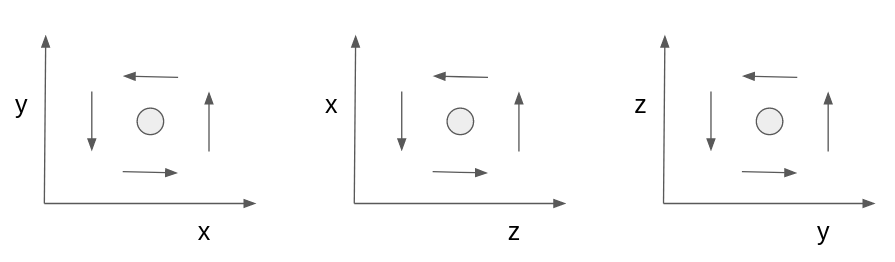
\includegraphics[width=15cm]{curl.png}
					\begin{center}
					Figure 1
				\end{center}
				
			\par \noindent In Figure 1's left graph, we've generalized what happens to a particle when a field induces positive curl. In these diagrams the arrows represent the field. We note that as \(x\) increases, the \(Q\) component of the field has a tendency to shift from negative to positive. Likewise as as \(y\) increases, the \(P\) component becomes more negative. In order to guarantee a positive value if the field is inducing a counter clockwise rotation we can  take the change of \(R\) with respect to \(y\) (which will be positive) and subtract from it the change of \(P\) with respect to \(y\) which will be negative. From this intuition, we get \(\frac{\partial Q}{\partial x} - \frac{\partial P}{\partial y}\) as the two dimensional curl.
			\newline
			\par\noindent In our analysis so far we've imagined that the field can only induce rotation on the \(xy\) plane. Because \(z\) is fixed in this scenario, the two dimensional curl is the \(\vec k\) component of the three dimensional curl. We can think of this as the observed rotation viewed from \(z\)'s perspective.
			\newline
			\par\noindent Looking again at Figure 1, the central diagram describes a hypothetical counter clockwise rotation from the perspective of \(y\). As \(z\) increases, the \(P\) component of the field becomes more positive and as \(x\) increases, the \(R\) compoment becomes more negative. So to guarantee a positive value we can write \(\frac{\partial P}{\partial z} - \frac{\partial R}{\partial x}\). The same analysis can be performed with Figure 1's right graph.
			

\section{Derivation of Two Dimension Curl}

	\begin{minipage}{.5\linewidth}		
		
		\par \noindent Suppose we have a patch of \(xy\) like the one described in Figure 2. We have here a simple connected region where the path \(C\) can be divided into \(C1 + C2 + C3 + C4\). We have also drawn here some vectors that approximate what the field \(F=<P,Q,R>\) is doing near these points along the four sub paths.
		\newline
		\newline
		So the line integral for the complete path is:
		\begin{flalign*}
			\oint_{C} \;F\;dr = \sum_{i=1}^{4} \int_{Ci}\;F\;dr
		\end{flalign*}
	
\end{minipage}
\begin{minipage}[c]{.5\linewidth}
	
	\begin{center}
		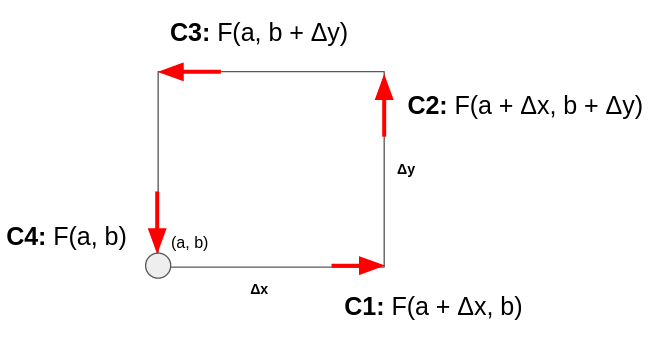
\includegraphics[width=8cm]{curl-deriv.png}
	\end{center}
	
	\begin{center}
		Figure 2
	\end{center}
	
\end{minipage}
\newline
\par\noindent For very small values of \(\Delta x\) and \(\Delta y\) we can state the following:
\newline
\begin{flalign*}
	\int_{C1} \; F\; dr \approx P(a + \Delta x, b) \Delta x \\
	\int_{C2} \; F\; dr \approx Q(a + \Delta x, b + \Delta y) \Delta y \\
	\int_{C3} \; F\; dr \approx P(a, b + \Delta y) \Delta x \\
	\int_{C4} \; F\; dr \approx Q(a, b) \Delta y 
\end{flalign*}
\par\noindent Our goal is ultimately to describe the rotational tendency of a field per area of \(\Delta x \Delta y\), albeit an infinitesimally small area. Our strategy here is to look at the horizontal (C1, C3) and vertical paths (C2, C4). Let's start with the horizontal:

\begin{flalign*}
 \lim_{(x,y) \rightarrow (0,0)} \frac{P(a + \Delta x, b) \Delta x - P(a, b+ \Delta x) \Delta x}{\Delta x \Delta y}
\end{flalign*}

\par\noindent Note how we treat C3 as a negative because it goes in the opposite direction of C1. Upon canceling out the \(\Delta x\) and evaluating the limit as x approaches zero we are left with:

\begin{flalign*}
	\lim_{y \rightarrow 0} \frac{P(a, b) - P(a, b+ \Delta y)}{\Delta y}
\end{flalign*}

\par\noindent If we modify this result by making it negative, we arrive at one of the two components of the two dimension curve:

\begin{flalign*}
	-\lim_{y \rightarrow 0}  \frac{P(a, b+ \Delta y) -P(a, b)}{\Delta y} = - \frac{\partial P}{\partial y}
\end{flalign*}
\newpage

\newpage

\par\noindent We can repeat this analysis for the vertical components:

\begin{flalign*}
	\lim_{(x,y) \rightarrow (0,0)} \frac{Q(a + \Delta x, b + \Delta y) \Delta y - Q(a, b) \Delta y}{\Delta x \Delta y}
\end{flalign*}

\par\noindent We take the limit as y approaches zero first and are left with the definition of a partial derivative with respect to \(x\), the remaining component of two dimension curl:

\begin{flalign*}
	\lim_{x \rightarrow 0} \frac{Q(a + \Delta x, b) - Q(a, b)}{\Delta x} = \frac{\partial Q}{\partial x}
\end{flalign*}





\section{Examples}
	\framebox{
		\parbox{\linewidth}{
			
			\textbf{Ex. 1} Calculate \(\nabla \times F\) given \(F(x,y,z) = \frac{1}{\sqrt{x^2+y^2+z^2}}(x\; \vec i + y\; \vec j + z\; \vec k)\)
			\newline
			\par\noindent Source:
			\newline
			\begin{flalign*}
				\frac{\partial R}{\partial y} =  \frac{zy}{2\sqrt{x^2+y^2+z^2}} \;\;\;
				\frac{\partial Q}{\partial z} =  \frac{zy}{2\sqrt{x^2+y^2+z^2}} \;\;\;
				\frac{\partial P}{\partial z} =  \frac{xz}{2\sqrt{x^2+y^2+z^2}} \\
				\frac{\partial R}{\partial x} =  \frac{xz}{2\sqrt{x^2+y^2+z^2}} \;\;\;
				\frac{\partial Q}{\partial x} =  \frac{xy}{2\sqrt{x^2+y^2+z^2}} \;\;\;
				\frac{\partial P}{\partial y} =  \frac{xy}{2\sqrt{x^2+y^2+z^2}}
			\end{flalign*}
		
			\begin{flalign*}
	\nabla \times F = (\frac{\partial R}{\partial y} - \frac{\partial Q}{\partial z}) \vec i\;\; +\;\; (\frac{\partial P}{\partial z} - \frac{\partial R}{\partial x})\vec j \;\; + (\frac{\partial Q}{\partial x} - \frac{\partial P}{\partial y})\vec k
			\end{flalign*}
		
			\begin{flalign*}
							\nabla \times F = 0\;\vec i + 0\;\vec j + 0\;\vec k
			\end{flalign*}
		
			\begin{center}
			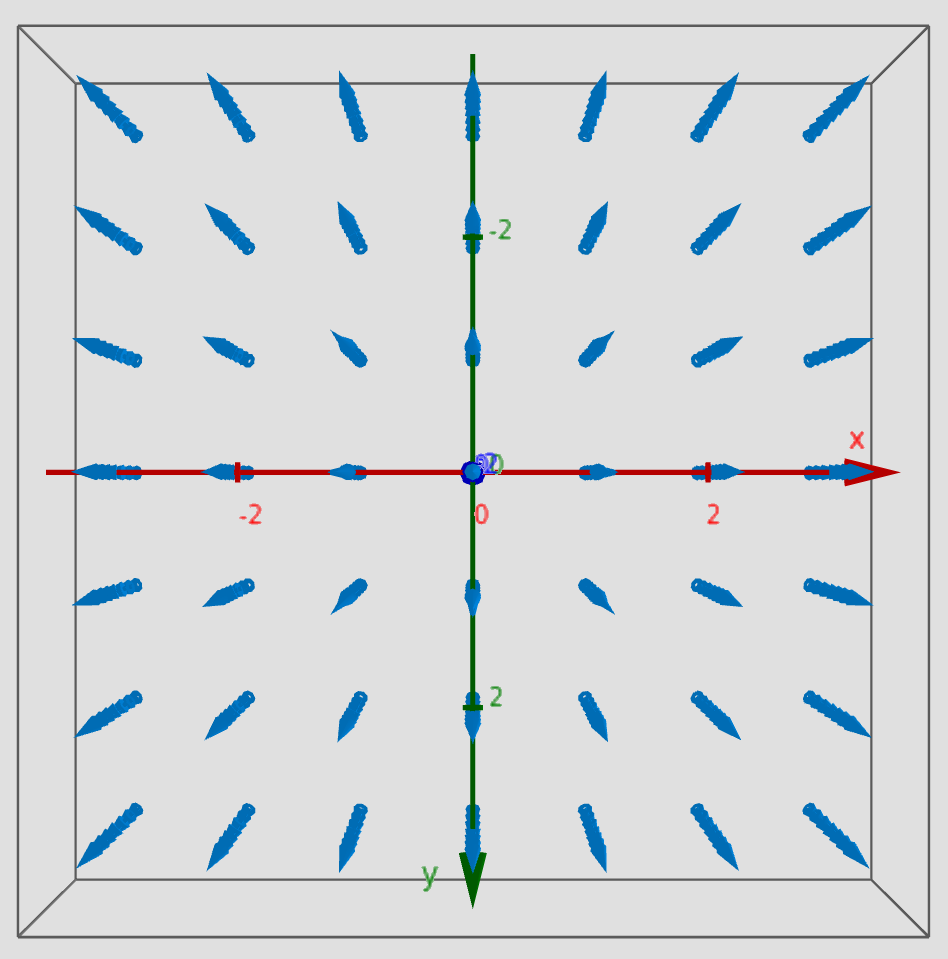
\includegraphics[width=7cm]{ex1field.png}
			\end{center}
			\begin{center}
				Figure 2
			\end{center}
		
		\par\noindent No curl is present. A graph of the field (top down) is shown in Figure 2. We can intuitively see that this field is incapable of inducing rotation.

		
	}
}
\newpage
	\framebox{
	\parbox{\linewidth}{
		
		\textbf{Ex. 2} Calculate \(\nabla \times F\) where \(F=xye^z\;\vec i + yze^x\;\vec k\)
		\newline
		
				\par\noindent Source:
				
			\begin{flalign*}
	\frac{\partial R}{\partial y} =  ze^x \;\;\;
	\frac{\partial Q}{\partial z} =  0 \;\;\;
	\frac{\partial P}{\partial z} =  xye^z \\
	\frac{\partial R}{\partial x} =  yze^x \;\;\;
	\frac{\partial Q}{\partial x} =  0 \;\;\;
	\frac{\partial P}{\partial y} =  xe^z
\end{flalign*}		
		
					\begin{flalign*}
			\nabla \times F = (\frac{\partial R}{\partial y} - \frac{\partial Q}{\partial z}) \vec i\;\; +\;\; (\frac{\partial P}{\partial z} - \frac{\partial R}{\partial x})\vec j \;\; + (\frac{\partial Q}{\partial x} - \frac{\partial P}{\partial y})\vec k
		\end{flalign*}
		
		\begin{flalign*}
			\nabla \times F = ze^x\;\vec i + xye^z - yze^x\;\vec j -xe^z\;\vec k
		\end{flalign*}
}}


\end{document}